\subsection{The target class cannot be duplicate with any imported class from different package after rename.}

If a class is imported from different package, we have to pre-check that the new name of the target class is not duplicate with the imported class after rename refactoring. 

\begin{figure}[th]
\centering
\begin{minipage}[t]{0.4\linewidth}
\begin{lstlisting}[language=java, basicstyle=\scriptsize\ttfamily,frame=single]
package q;
import p.C;

class A{
}

class B{
} 
\end{lstlisting}
\centering(a) Before
\end{minipage}
\hfill
\begin{minipage}[t]{0.4\linewidth}
\begin{lstlisting}[language=java, basicstyle=\scriptsize\ttfamily,frame=single]
package q;
import p.C;

class A{
}

class C{
} 
\end{lstlisting}
\centering(b) After
\end{minipage}
\caption{\textbf{RcR from B to C}}
\label{figure:fig2}
\end{figure}

In Fig. \ref{figure:fig2} (a), we see that class B is not duplicate with class A and we can implement RcR on class B to any other name except `A' as mentioned in section \ref{sec:precon1}. However, in Fig. \ref{figure:fig2} (b), when we try to implement RcR from \emph{B to C}, Java compiler produces an error \textit{``a compilation unit must not import and declare a type with the same name''}~\cite{EclipseWebPage} as shown in Fig. \ref{figure:comperr}. This is because the compiler cannot distinguish between the \emph{imported class C} of package `p' and the \emph{existing class C} of package `q'. 

\begin{figure}[H]
\centerline{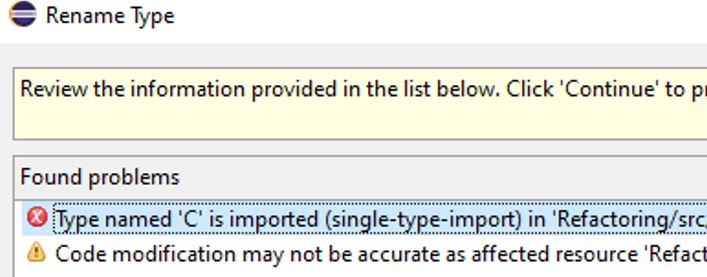
\includegraphics[width=85mm,scale=0.5]{CUE.jpg}}
\caption{\textbf{Compilation Unit Error} }
\label{figure:comperr}
\end{figure}

Therefore, it is essential to pre-check that the target class should not have duplicate name with any of imported class after RcR.


As mentioned in  section \ref{sec:precon2}, the same precondition also holds good for renaming a child class. Suppose a Java file has a class and its children classes as shown in Fig. \ref{figure:figpc3_1}. We see that if parent class A imports a class C from package `p' and if we try to rename the child class from B to C or D to C, Java compiler produces an error as ``C is already defined''.This precondition is applicable for all ancestor class and we have to trace back and check if any of the parent class is importing a class with same name before renaming the child class within the same java file.

\begin{figure}[th]
\centering
\begin{minipage}[t]{0.45\linewidth}
\begin{lstlisting}[language=java, basicstyle=\scriptsize\ttfamily,frame=single]	
//A.java

package q;
import p.C;

public class A{	
}

class B extends A{	
}

class D extends B{
}
\end{lstlisting}
\centering{(a) Before}
\end{minipage}
\hfill
\begin{minipage}[t]{0.45\linewidth}
\begin{lstlisting}[language=java, basicstyle=\scriptsize\ttfamily,frame=single]
//A.java

package q;
import p.C;

public class A{	
}

class C extends A{	
}

class D extends B{
}	
\end{lstlisting}
\centering{(b) After}
\end{minipage}
\caption{\textbf{RcR from B to C}}
\label{figure:figpc3_1}
\end{figure}

If a parent class imports a class from different package and if the child class is defined in a separate java file, then in that case we can refactor and rename the child class to the imported class name.
